\documentclass{article}%

\usepackage{amsmath}%
\usepackage{graphicx}
\usepackage[english,greek]{babel}
\usepackage[utf8x]{inputenc}
\usepackage{listings}
\usepackage{lipsum}

\newcommand{\exedout}{%
  \rule{0.8\textwidth}{0.5\textwidth}%
}



\begin{document}

\selectlanguage{greek}

\title{Δίκτυα Επικοινωνιών\\2η εργαστηριακή άσκηση}
\author{Γεώργιος Δασούλας\\Α.Μ: 03112010 \\ 6ο Εξάμηνο 2014-2015  }
\date{\today}
\maketitle

\textbf{{\underline{1.Συνθετότερα προβλήματα με το  \textlatin{NS2} }}} \\

Στο πρώτο μέρος της Άσκησης 2 ορίζουμε στο \textlatin{NS2} µια τοπολογία δικτύου µε τέσσερις κόµβους, στην
οποία ένας κόµβος λειτουργεί ως δροµολογητής και προωθεί τα δεδοµένα που στέλνουν δύο κόµβοι στον
τέταρτο κόµβο.
\begin{figure}[htbp]
	\centering
		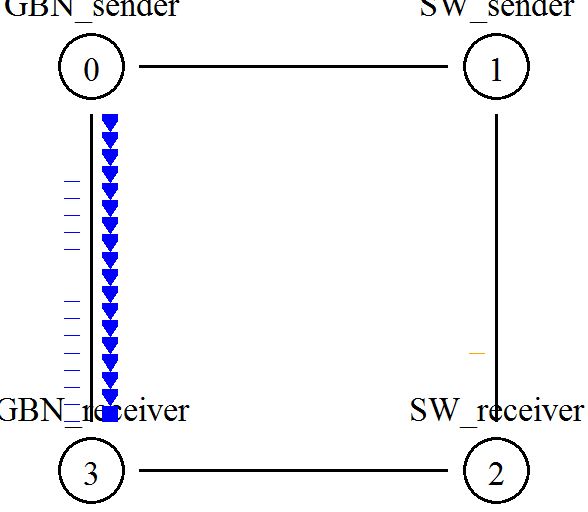
\includegraphics[width=0.40\textwidth]{../../Desktop/1.png}
	\label{fig:1}
\end{figure}

Από το \textlatin{animation} παρατηρούμε πως από κάποια στιγμή και μετά ο δρομολογητής στον κόμβο 2 απορρίπτει πακέτα.Αυτό οφείλεται στο ότι ο συνολικός αριθμός πακέτων που στέλνονται από τους κόμβους 0 , 1 στον κόμβο 2 είναι μεγαλύτερος από το εύρος ζώνης της ζεύξης μεταξύ των κόμβων 2,3.Συγκεκριμένα , η χωρητικότητα της ζεύξης των κόμβων 2,3 είναι $2 Mbits/sec * 10 msec = 20000 bits$ , άρα, $\frac{20000}{8}=2500$ \textlatin{bytes}. Όμως , λόγω των πακέτων που στέλνουν οι κόμβοι 0,1 θα έπρεπε στη ζεύξη να υπάρχουν $\frac{1000 bytes}{0.005}*0.01sec + \frac{1000 bytes}{0.008} * 0.01sec = 2000+ 1250 = 3250$ \textlatin{bytes}. Άρα, βλέπουμε ότι αναγκαστικά στον κόμβο 2 πρέπει να χαθούν πακέτα, όταν θα ξεκινήσει η ταυτόχρονη αποστολή πακέτων από τους δύο κόμβους. \newpage


\textbf{{\underline{1.3 Σημάδεμα ροών  }}} \\\\
Και οι δύο ροές παριστάνονται µε µαύρο χρώµα, οπότε ο µόνος τρόπος να διαπιστωθεί τι συµβαίνει στα
πακέτα είναι να τα παρακολουθεί κάποιος στο $NAM$ κάνοντας κλικ πάνω τους.Αυτό που θα κάνουμε στη συνέχεια είναι να ορίσουμε με διαφορετικά χρώματα τις δύο ροές πακέτων.

\begin{figure}[htbp]
	\centering
		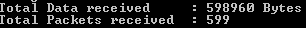
\includegraphics[width=0.40\textwidth]{../../Desktop/2.png}
	\label{fig:2}
\end{figure}

Προσθέτουμε τώρα μια ουρά αναμονής για να μπορούμε να βλέπουμε τα πακέτα που απορρίπτονται.Παρατηρούμε πως απορρίπτονται μόνο κόκκινα πακέτα.


\begin{figure}[htbp]
	\centering
		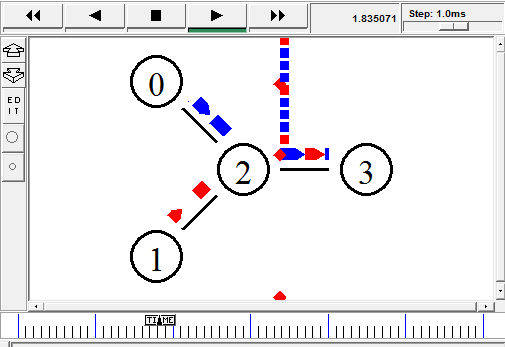
\includegraphics[width=0.40\textwidth]{../../Desktop/3.png}
	\label{fig:3}
\end{figure}

Για να βελτιώσουμε την ουρά αναμονής χρησιµοποιούμε µια ουρά $SFQ$
\textlatin{(Stochastic Fair Queuing)} για τη ζεύξη από “$n2$” προς “$n3$”.Βλέπουμε ότι τώρα απορρίπτονται μόνο μπλε πακέτα κι αυτό οφείλεται στό ότι τα κόκκινα πακέτα μεταδίδονται με ρύθμο που συμφωνεί με αυτόν που της παραχωρείται από την $SFQ$. 
\begin{figure}[htbp]
	\centering
		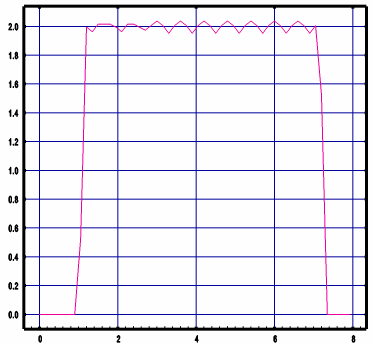
\includegraphics[width=0.40\textwidth]{../../Desktop/4.png}
	\label{fig:4}
\end{figure}
\newpage

\textbf{{\underline{1.5 Παρακολούθηση ουράς µε το \textlatin{Xgraph}}}} \\\\
Παρακάτω βρίσκονται οι γραφικές σε $Droptail$ και $SFQ$ αντίστοιχα.Στο κάθε διάγραμμα , η μπλε γραμμή δείχνει την πρώτη ροή μπλε πακέτων , ενώ η κόκκινη γραμμή τη ροή των κόκκινων πακέτων.

\selectlanguage {english}
\begin{figure}[htbp]
	\centering
		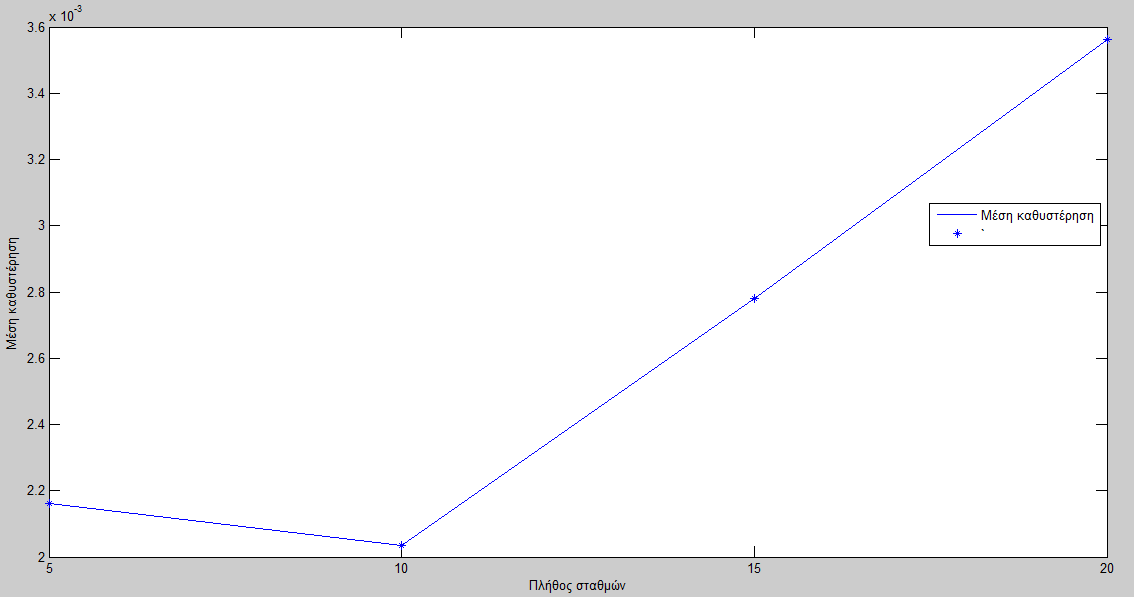
\includegraphics[width=0.50\textwidth]{../../Desktop/5.png}
	\caption{Droptail}
\end{figure}
\begin{figure}[htbp]
	\centering
		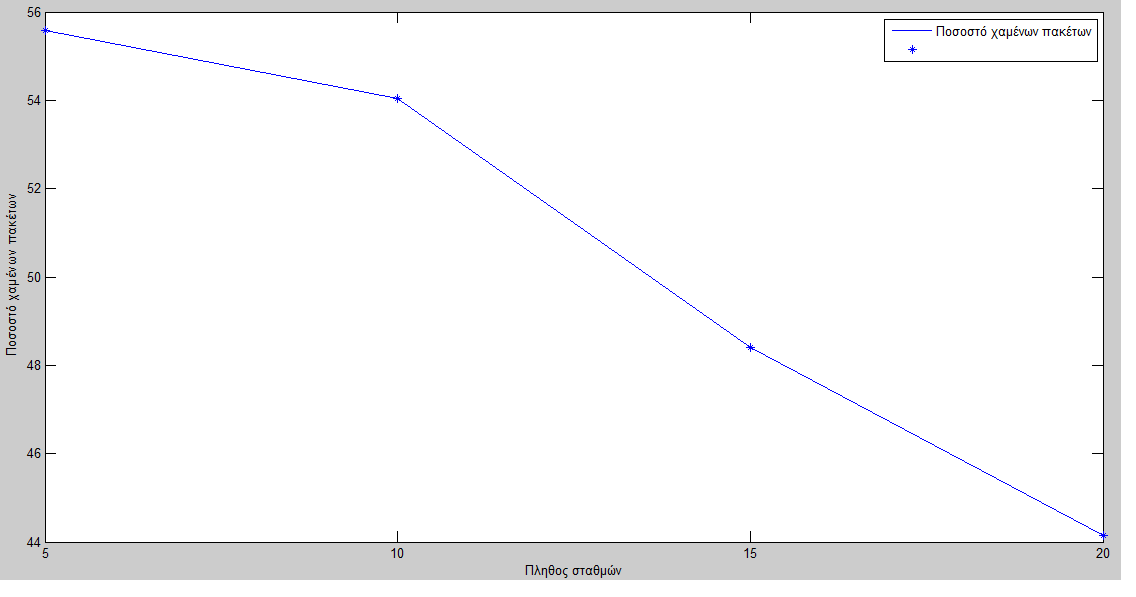
\includegraphics[width=0.50\textwidth]{../../Desktop/6.png}
	\caption{SFQ}
\end{figure}

\selectlanguage{greek}

\textbf{1.6 Ερωτήσεις} \\\\
\textsl{\textbf{\underline{{Απαντήσεις ερωτήσεων}}}}
\begin{itemize}
	\item Ποια είναι η µέγιστη τιµή του ρυθµού µεταφοράς των δεδοµένων για τις δυο ροές, όπως προκύπτει
από τις γραφικές παραστάσεις του $Xgraph$ (για ουρά $DropTail$ και ουρά $SFQ$);\\
\textbf{Απάντηση}: Για \textlatin{Droptail} , όπως φαίνεται από τις γραφικές , τα μπλε πακέτα έχουν μέγιστο ρυθμό μεταφοράς 1.64 $Mbits/sec$, ενώ τα κόκκινα πακέτα έχουν μέγιστο ρυθμό μεταφοράς 1.6 $Mbits/sec$. \\Αντίστοιχα, για $SFQ$ έχουμε για τα μπλε μέγιστο 1.6 $Mbits/sec$ , ενώ για τα κόκκινα 1.04 $Mbits/sec$. \\
\item Ποια είναι η ελάχιστη τιµή του ρυθµού µεταφοράς των δεδοµένων για τις δυο ροές, στο διάστημα
που αποστέλλουν δεδομένα και οι δύο πηγές, για κάθε τύπο ουράς;\\ 
\textbf{Απάντηση}: Και πάλι από τις γραφικές φαίνεται πως για $Droptail$ έχουμε ελάχιστο ρυθμό μεταφοράς για όσο χρονικό διάστημα αποστέλλονται και από τις δύο πηγές  για τα μπλε 1 $Mbit/sec$ ενώ για τα κόκκινα πακέτα $0.4$ $Mbits/sec$ , ενώ για $SFQ$ έχουμε ελάχιστο τόσο για τα μπλέ , όσο και τα κόκκινα 1 $Mbits/sec$ . \\
\item Ποιο είναι το μέγιστο ποσοστό των πακέτων που χάνονται από την µπλε και κόκκινη ροή για τους
δύο τύπους ουρών; Ποιες είναι οι μέγιστες απώλειες κάθε ροής σε $bit/sec$;\\
\textbf{Απάντηση}:Οι μέγιστες απώλειες προκύπτουν από τη διαφορά του μέγιστου ρυθμού μεταφοράς και του ελάχιστου. Άρα, για ουρά τύπου $DropTail$ έχουμε πως για τα μπλε πακέτα οι μέγιστες απώλειες είναι $1.64-1=0.64 Mbits/sec$,άρα το μέγιστο ποσοστό απωλειών είναι $\frac{0.64}{1.64}=39.02\%$, ενώ για τα κόκκινα πακέτα οι μέγιστες απώλειες είναι $1.6-0.4=1.2 Mbits/sec$, άρα το μέγιστο ποσοστό απωλειών είναι $\frac{1.2}{1.6}=75\%$.\\Αντίστοιχα,για ουρά τύπου $SFQ$ έχουμε για τα μπλε πακέτα πως οι μέγιστες απώλειες είναι $1.6-1=0.6 Mbits/sec$, άρα το μέγιστο ποσοστό απωλειών είναι $\frac{0.6}{1.6}=37.5\%$ , ενώ για τα κόκκινα πακέτα ισχύει πως οι μέγιστες απώλειες είναι $1.04-1=0.04 Mbits/sec$, άρα μέγιστο ποσοστό απωλειών $\frac{0.04}{1.04}=3.84\%$.\\ 

\item Είναι τα ποσοστά αυτά αναμενόμενα, αν λάβουμε υπόψη τον ρυθμό μετάδοσης κάθε πηγής, τη
χωρητικότητα των ζεύξεων και τον τύπο ουράς;\\\\
\textbf{Απάντηση}:Παρατηρούμε πως η αλλαγή του τύπου ουράς από $Droptail$ σε $SFQ$ βελτιώνει τη ροή των κόκκινων πακέτν, καθώς μειώνεται αισθητά το μέγιστο ποσοστό των πακέτων που απορρίπτει ο κόμβος 2.Το $DropTail$ λειτουργεί με πολιτική $FIFO$ , οπότε η συχνότερη ροή των μπλε πακέτων ωθεί στην απόρριψη των κόκκινων πακέτων , κάτι που δε συμβαίνει στην περίπτωση ουράς τύπου $SFQ$.Το ποσοστό των πακέτων που απορρίπτονται στον κόμβο 2 ( καθορίζεται από τη χωρητικότητα της ζεύξης) ισούται με  $\frac{3250-2500}{3250}=23.08\%$. Χρησιμοποιώντας τα δεδομένα των γραφικών παραστάσεων βρίσκουμε ότι με $Droptail$ ανά πάσα στιγμή απορρίπτονται το πολύ $2000*39.02\% =780.4$ \textlatin{bytes} μπλε πακέτων και το πολύ $1250*75\%=937.5$ \textlatin{bytes} κόκκινων πακέτων, ενώ με $SFQ$ ανα πάσα στιγμή απορρίπτονται το πολύ $2000*37.5\%=750$ \textlatin{bytes} μπλε πακέτων και το πολύ $1250*3.84\%=48$ \textlatin{bytes} κόκκινων πακέτων.Θεωρητικά , όπως είδαμε παραπάνω λόγω της χωρητικότητας της ζεύξης απορρίπτονται $3250-2500=750$ \textlatin{bytes} πακέτων συνολικά.Αν αθροίσουμε , λοιπόν τις αντίστοιχες απώλειες για $DropTail$ και $SFQ$ , βλέπουμε πως η ουρά τύπου $SFQ$ βελτιώνει σημαντικά τη ροή των δεδομένων προσεγγίζοντας τα θεωρητικά ποσοστά απωλειών. \\
\item Επαληθεύστε τις απαντήσεις της Ενότητας 1.5 (για ουρά $DropTail$ και ουρά $SFQ$), χρησιµοποιώντας
τις γραφικές παραστάσεις του $Xgraph$.\\  
\textbf{Απάντηση}:	H ερώτηση απαντάται στο παραπάνω ερώτημα\\
\item  Στις γραφικές παραστάσεις του $Xgraph$ υπάρχουν διαστήματα με μηδενικό ρυθμό μετάδοσης και
διαστήματα που η μια ροή από μόνη της ξεπερνά τον καθορισμένο ρυθμό μετάδοσης της αντίστοιχης
πηγής στη ζεύξη 2-3. Πώς ερμηνεύετε αυτή τη συμπεριφορά για κάθε τύπο ουράς;\\
 \textbf{Απάντηση}:Τα διαστήματα με μηδενικό ρυθμό μετάδοσης είναι διαστήματα , που κανένας από τους δύο κόμβους δεν στέλνει πακέτα στον κόμβο ζεύξης. Επίσης , για ουρά τύπου $DropTail$ ,επειδή η ροή των μπλε πακέτων σταματάει πριν σταματήσει και η ροή των κόκκινων πακέτων, σημαίνει πως για κάποιο διάστημα θα προστίθενται στην ουρά μόνο κόκκινα πακέτα και έτσι θα έχουμε πακέτα της μίας ροής μόνο που περιμένουν έτοιμα να κυκλοφορήσουν και θα ξεκινήσουν με μεγαλύτερη ταχύτητα από την πηγή που τα στέλνει.\\

\end{itemize}

\textbf{{\underline{2. Δυναμική συμπεριφορά δικτύου }}} \\

Στο δεύτερο μέρος της Άσκησης 2 παρουσιάζεται ένα παράδειγµα δυναµικού δικτύου, όπου η
δροµολόγηση αναπροσαρµόζεται όταν κοπεί κάποια ζεύξη. Κατά την πορεία δείχνουμε πώς
µπορούμε  να διατηρήσουμε ένα µεγαλύτερο αριθµό κόµβων σε ένα $Tcl$ $array$ αντί να δώσουμε σε κάθε κόµβο
το δικό του όνομα. \\

\newpage
\textbf{{\underline{2.1 Δηµιουργία µεγαλύτερης τοπολογίας }}} \\
Αυτή τη φορά επειδή θέλουμε να κατασκεύασουμε μεγαλύτερες τοπολογίες με περισσότερους κόμβους και περισσότερες ζεύξεις , χρησιμοποιύμε βρόχους $for$ , για να δηλώσουμε τα αντίστοιχα μεγέθη στον κώδικα . Παρακάτω, βρίσκεται μια κυκλική τοπολογία 10 κόμβων.Βλέπουμε πακέτα να μεταφέρονται από τον κόμβο 0 στον κόμβο 4.
\begin{figure}[htbp]
	\centering
		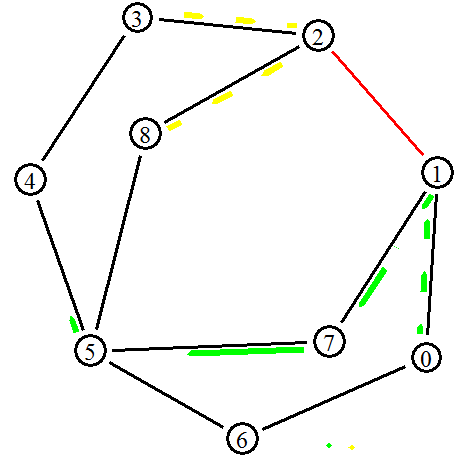
\includegraphics[width=0.40\textwidth]{../../Desktop/7.png}
	\label{fig:7}
\end{figure}

\textbf{{\underline{2.2 Διακοπή ζεύξης }}} \\\\
Βλέπουμε, τώρα ότι με την διακοπή ζεύξης στο διάστημα $ 1.5 -3.0 sec$ , οι πληροφορίες χάνονται σε αυτό το διάστημα.Χρησιμοποιούμε τη δυναμική δρομολόγηση για να λύσουμε αυτό το πρόβλημα, μεταβάλλοντας κατάλληλα το τμήμα κώδικα $tcl$. Με τη δυναμική πλέον δρομολόγηση βλέπουμε ότι , τα πακέτα μεταφέρονται από άλλο δρόμο ($ 9 -> 8 ->7->6->5->4$) για όσο χρονικό διάστημα διακόπτεται η ζεύξη των κόμβων 2,3. Αν χαμηλώσουμε αρκετά ταχύτητα στο $NAM$ μπορούμε να δούμε ότι υπάρχουν πακέτα “$rtProtoDV$” (\textlatin{routing protocol distance vector}) τα οποία
χρησιµοποιούνται για την ανταλλαγή πληροφορίας δροµολόγησης µεταξύ των κόµβων.
\begin{figure}[htbp]
	\centering
		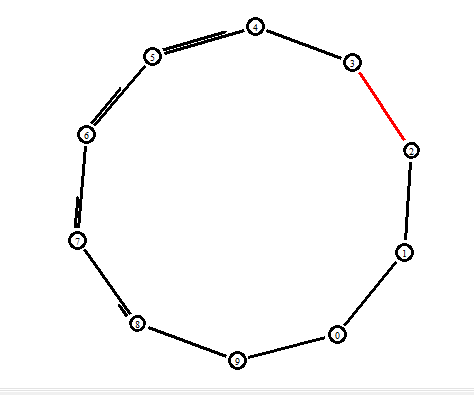
\includegraphics[width=0.50\textwidth]{../../Desktop/8.png}
	\label{fig:8}
\end{figure}

\newpage

\textbf{{{2.3 Ερωτήσεις }}} \\
\textsl{\textbf{\underline{{Απαντήσεις ερωτήσεων}}}}\\
\begin{itemize}
	\item Περιγράψτε µε απλά λόγια τη διαδικασία που έλαβε χώρα στο παραπάνω \textlatin{animation}. Από τι
εξαρτάται η δυναμική συμπεριφορά του δικτύου;\\
\textbf{Απάντηση}:Για τη δυναμική συμπεριφορά του δικτύου χρησιμοποιούμε πακέτα πρωτοκόλλου $rtProtoDV$, τα οποία ενημερώνουν για τους τρόπους δρομολόγησης. Έτσι, μέχρι το $1.5sec$ χρησιμοποιείται το συντομότερο μονοπάτι για δρομολόγηση, και μετά το $1.5 sec$ και από τη στιγμή που ενημερώσουν τα πακέτα $rtProtoDV$ τον κόμβο 0 ότι αφαιρείται η ζεύξη $2-3$ , αλλάζει η δρομολογήση προς την αντίθετη κατεύθυνση εφόσον πρόκειται για κυκλική δικτύωση. \\
\item Γιατί ο κόµβος 0 συνεχίζει να στέλνει πακέτα στον κόµβο 2 για κάποια $msecs$ ενώ έχει πέσει η
σύνδεση µεταξύ των κόµβων 2 και 3;
\textbf{Απάντηση}:Όπως απαντήσαμε και στην προηγούμενη ερώτηση , μέχρι να ενημερώσουνα τα πακέτα $rtProtoDV$ τον κόμβο 0 , ο $UDP$ $agent$ δε γνωρίζει ότι υπάρχει διακοπή ζεύξης και συνεχίζει να στέλνει πακέτα.Από το \textlatin{animation} παρατηρούμε πως από τη στιγμή που διακοπεί η ζεύξη μέχρι να γίνει αλλαγή κατεύθυνσης μεσολαβούν περίπου $50msec$.\\
\item Για ποιο λόγο σταµατάει και αλλάζει τη δροµολόγηση προς τον κόµβο 9;
\textbf{Απάντηση}:Σταματάει και αλλάζει κατεύθυνση προς τον κόμβο 9 ακριβώς για να βρει άλλο τρόπο να στείλει τα πακέτα πληροφορίας στον κόμβο 4 και εκμεταλλεύται την κυκλικότητα του δικτύου.\\

\end{itemize}


\textbf{{\underline{2.4 Προσοµοίωση στο $Xgraph$ }}} \\
Η προσομοίωση με το $Xgraph$ δίνει το παρακάτω αποτέλεσμα :
\begin{figure}[htbp]
	\centering
		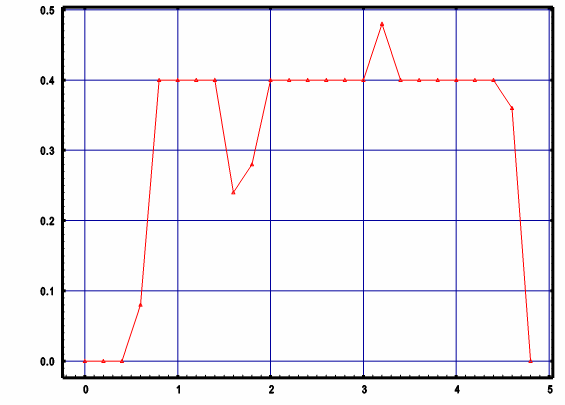
\includegraphics[width=0.55\textwidth]{../../Desktop/9.png}
	\label{fig:9}
\end{figure}

\newpage

\textbf{2.5 Ερωτήσεις } \\
\begin{itemize}
	\item Συγκρίνετε το \textlatin{animation} µε τη γραφική παράσταση. Είναι κατά τη γνώµη σας σωστό το γράφηµα;\\
	\textbf{Απάντηση}:Χοντρικά το γράφημα είναι σωστό. Λόγω της χαμηλής ακρίβειας του γραφήματος (μεγάλος χρόνος καταγραφής) δε φαίνεται η καθυστέρηση της αλλαγής δρομολόγησης μέχρι να ενημερωθεί ο κόμβος 0.\\
	\item Προσπαθήστε να το βελτιώσετε αλλάζοντας µία από τις µεταβλητές της διαδικασίας “\textlatin{record}”. Να
σχεδιάσετε, με το $Xgraph$, δύο βελτιωμένα γραφήματα για δύο διαφορετικές τιμές της μεταβλητής
που θα αλλάξετε. \\
	\textbf{Απάντηση}:	Για τη βελτίωση της ακρίβειας του γραφήματος , πρέπει να μειώσουμε το χρόνο δειγματοληψίας (λήψης στιγμιοτύπων), ώστε οι μικρές αλλαγές να είναι παρατηρήσιμες.Αυτό που πρέπει να αλλάξουμε είναι συνεπώς :
	\textlatin{set time 0.2}. Ακολουθούν 2 γραφήματα με αντίστοιχους χρόνους δειγματοληψίας : $t=0.1 sec$ και $t=0.04 sec$. 
	\selectlanguage{english}

\begin{figure}[htbp]
\centering
\begin{minipage}{0.45\textwidth}
\centering
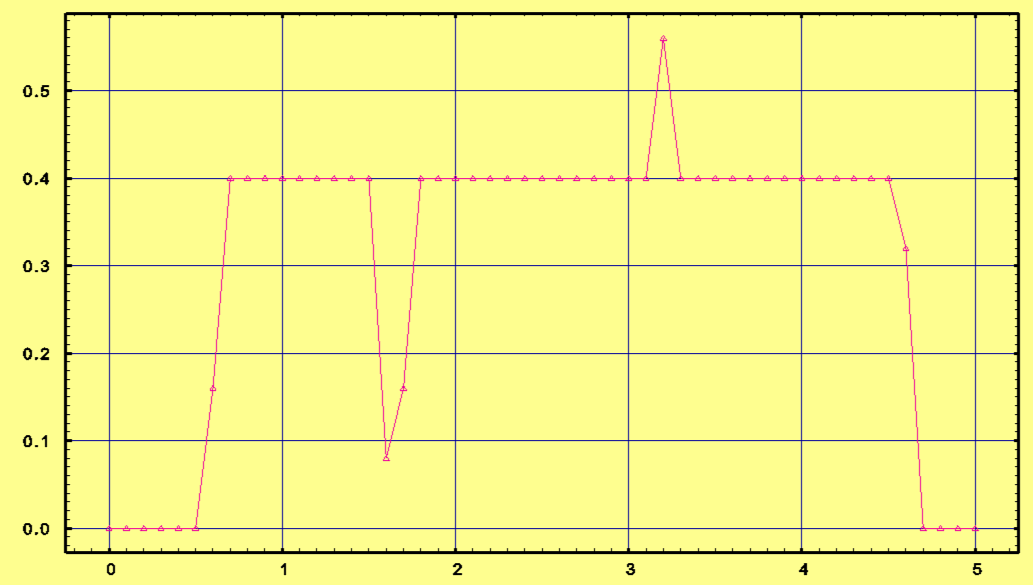
\includegraphics[width=1.00\textwidth]{../../Desktop/10.png}
\caption{t=0.1 sec}
\end{minipage}\hfill
\begin{minipage}{0.45\textwidth}
\centering
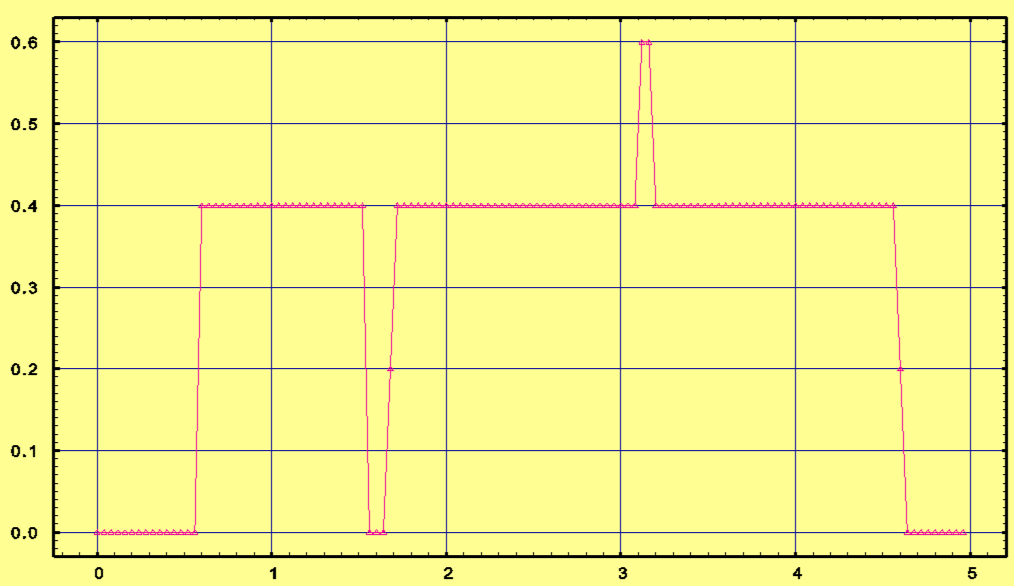
\includegraphics[width=1.00\textwidth]{../../Desktop/11.png}
\caption{t=0.04 sec}
\end{minipage}
\end{figure}


\selectlanguage{greek}
	\item  Ποιος είναι ο μέγιστος ρυθμός άφιξης δεδομένων στον κόμβο n(4); Είναι αναμενόμενη αυτή η τιμή,
με δεδομένο το ρυθμό μετάδοσης της πηγής στον κόμβο n(0); Αιτιολογείστε γιατί συμβαίνει αυτό,
παραθέτοντας ένα κατάλληλο στιγμιότυπο από το NAM\\
	\textbf{Απάντηση}: Όπως φαίνεται από τη γραφική παράσταση, στον κόμβο 4 έχουμε διπλάσιο ρυθμό μετάδοσης από αυτόν του κόμβου 0 που φτάνει στα $0.8 Mbits/sec$, που είναι και ο μέγιστος ρυθμός. Αυτό οφείλεται στο ότι μόλις επανέλθει η ζεύξη $2-3$ θα έχουμε πλέον δύο ροές πακέτων . Αυτό φαίνεται και στο παρακάτω \textlatin{animation}. 
	\begin{figure}[htbp]
		\centering
			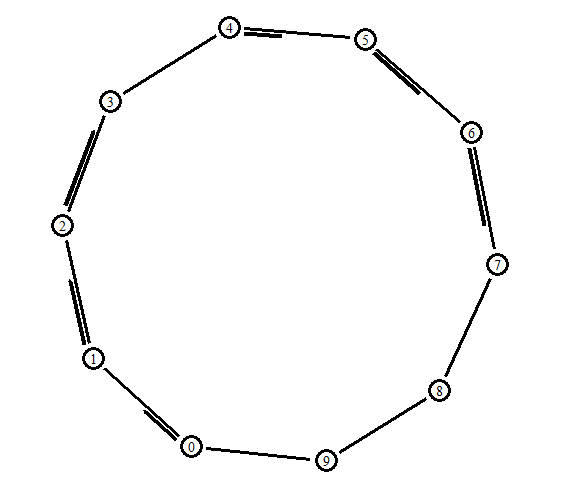
\includegraphics[width=0.50\textwidth]{../../Desktop/12.png}
		\label{fig:12}
	\end{figure}
	 \newpage
	\item Εξηγήστε το σχήµα της γραφικής παράστασης σε συνάρτηση µε τα γεγονότα και τις παραµέτρους
του δικτύου. \\
	\textbf{Απάντηση}:H περιγραφή της γραφικής παραστάσης σε συνάρτηση με τα γεγονότα και τις παραμέτρους του δικτύου έχει δοθεί παραπάνω. Αξίζει να τονισθεί πως για χρόνο μεγαλύτερο των $3 sec $ έχουμε από τον κόμβο 0 διπλή αποστολή πακέτων προς τον κόμβο 4 με δύο διαφορετικές διαδρομές και κατά συνέπεια ο ρυθμός μετάδοσης του κόμβου 4 για κάποιο μικρό χρονικό διάστημα είναι διπλάσιος από το ρυθμό μετάδοσης του κόμβου 0.Για χρόνο μεγαλύτερο των $4.5 sec$ έχουμε συνεχή μείωση του ρυθμού μετάδοσης , καθώς σταματάει η αποστολή πακέτων από τον κόμβο 0 .\\

\end{itemize}











\end{document}